\scanpage{71}
\mspage{\handwritten{- 6 -}}
\deleted{mis} mis en lumière (c'est mieux expliqué dans XIV 5.1 et 5.2) ; la référence (V 3.3.2) est vide.

p.18, li.3 : supprimer ``commutatifs''.

p.18, li.5 du bas : ``qu'on laisse au lecteur le soin d'écrire''.

p.19, li.3 : est-ce vraiment possible sans autre hypothèse sur $Z$ ?

p.19, li.7 : ``linéairement'' = ``rationnellement'' ?

p.19, li.15 : ``standard'' et non ``standart''.

p.19, li.11 du bas : ``une conjecture équivalente ...'' : on utilise implicitement le fait que $\mathrm{Gr}^{\bullet}\handwritten{\xrightarrow{\sim}}\mathrm{Gr}^{\bullet}_{\mathrm{top}}$ modulo torsion (VII\hspace{2em}).

p.19, li.3 du bas : référer à (SGA 5 IV\hspace{2em}).

p.20, li.10 : référer à (EGA IV 2.8) pour $Z$ plat sur $S$. Il faudrait aussi une référence pour le fait que $\dim(Z_s) = \dim(Z_t)$.

p.20, li.16 : ``rationnelle'' et non ``rationelle''. De même, 2 lignes plus bas, ``rationnellement'' et non ``...''. N'est-il pas prudent de supposer $f$ lisse ?

% Two faint detached traces above the final e; authorship and function unresolved.
p.20, li. 3 du bas : manque flèch\makebox[0pt][l]{\hspace{0.05em}\raisebox{2.0ex}{\parbox{0.8em}{\figure{\unsure{\begin{tikzpicture}[x=1mm,y=1mm,baseline=0pt]
\fill[gray!65] (0,0) ellipse[x radius=0.28,y radius=0.12,rotate=12];
\fill[gray!65] (0.62,1.03) ellipse[x radius=0.12,y radius=0.34,rotate=-9];
\end{tikzpicture}}}}}}e.

p.22, li.8 : ``On peut donc prendre (cf. IV 2.12) ...''.

p.2\deleted{\unsure{2|3}}2, li.5 : Supposer $X$ plat sur $S$.

p.23, li.2 : hypothèses sur $X$ ?

p.23, dernière ligne : donner le corollaire pour $\mathrm{NS}$ ?

% Short detached stroke in the left margin, immediately before the p.24 entry.
\noindent\makebox[0pt][l]{\hspace{-0.66cm}\raisebox{0.8ex}{\parbox{0.66cm}{\handwritten{\figure{\begin{tikzpicture}[x=1mm,y=1mm,baseline=0pt]
\draw[line width=0.4pt] (0,0) .. controls (2.0,0.23) and (4.3,0.25) .. (6.2,0.04);
\end{tikzpicture}}}}}}p.24, li.3 : supprimer ``localement''(canular à la li. 11).

p.24, li.6 : ``on note (EGA II 7.1.9) ...''.

% The points after et are slanted and elevated; no colon value or writing operation is asserted.
p.24, li.11 : références pour ``essentiellement de type fini'' et \hspace{0.35em}\raisebox{0.7ex}{\parbox{0.7em}{\figure{\unsure{\begin{tikzpicture}[x=1mm,y=1mm,baseline=0pt]
\fill (0,0) ellipse[x radius=0.18,y radius=0.15];
\fill (0.55,0.80) ellipse[x radius=0.13,y radius=0.22,rotate=-24];
\end{tikzpicture}}}}} ``universellement japonais'' ?

% Long left-margin stroke with a return loop reaching beneath the p.24 prefix.
\noindent\makebox[0pt][l]{\hspace{-3.10cm}\raisebox{-2.6mm}{\parbox{3.65cm}{\handwritten{\figure{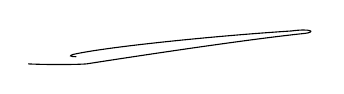
\begin{tikzpicture}[x=1mm,y=1mm,baseline=0pt]
\draw[line width=0.4pt] (0,0) .. controls (2.0,-0.10) and (5.6,-0.12) .. (7.4,0)
 .. controls (14.6,1.12) and (28.1,3.15) .. (35.2,3.88)
 .. controls (36.5,4.05) and (36.0,4.53) .. (33.4,4.18)
 .. controls (24.0,3.58) and (10.0,2.18) .. (5.7,1.20)
 .. controls (5.25,1.06) and (5.15,0.94) .. (6.10,0.91);
\end{tikzpicture}}}}}}p.24, dernière ligne : dommage qu'on ne do\deleted{t}n\deleted{\unsure{e|a}}ne pas de \deleted{\unsure{m}}démonstration.

p.25, li.8 : ``le soin de'' et non ``de''. Répétition \deleted{\unsure{malsonnante}} de ``développer''.

p.25, li.13 du bas : ``on peut construire $S'$ '' et non ``... $S$''

% archive sheet number: 70
